\documentclass[10pt,a4paper]{article}
\usepackage[utf8]{inputenc}\DeclareUnicodeCharacter{2212}{-}
\usepackage{graphicx,wrapfig,lipsum}
\usepackage[T1]{fontenc}
\usepackage{float}
\usepackage[table,xcdraw]{xcolor}
\usepackage[polish]{babel}
\usepackage{wrapfig} 
\usepackage{caption}
\usepackage{subcaption}
\usepackage{mathtools}
\usepackage{lmodern}
\usepackage{enumitem}
\usepackage{lscape}
\usepackage{url}
\usepackage{longtable}
\usepackage[version=4]{mhchem}
\usepackage{mathpazo}
\usepackage{booktabs}
\usepackage{pgf}


\author{Wojciech Noskowiak}
\title{Raport z ćwiczenia L9}
\date{Sierpień 2021}

\usepackage{natbib}
\usepackage{graphicx}

\begin{document}

\maketitle
\tableofcontents

\begin{abstract}
    Zbadałem stężenie dwutlenku azotu w próbkach powietrza pobranych z otoczeń różnych wyładowań elektrycznych w oparciu o metodę SSWO. W tym celu dopasowałem odpowiednie krzywe do uzyskanych eksperymentalnie danych. Większość uzyskanych przez mnie danych okazała się być miarodajna. Część uzyskanych przez mnie wyników okazała się być niezgodna z przewidywaniami teoretycznymi.
\end{abstract}

\newpage

\addcontentsline{toc}{section}{Wstęp}
\section*{Wstęp}
Celem ćwiczenia było zbadanie stężenia $\text{NO}_{\text{2}}$ w próbkach powietrza pobranych z otoczeń różnych wyładowań elektrycznych. Do tego celu wykorzystano w ćwiczeniu metodę SSWO. Wartości stężeń uzyskałem poprzez analizę dostarczonych mi wyniki pomiarów eksperymentalnych. Przekazane mi dane przebadałem w oparciu o polecenia z instrukcji \cite{instrukcja}, materiały dostępne na stronie pracowni \cite{strona} oraz dokumenty przekazane przez prowadzącego ćwiczenie \cite{sswo}. Przekazane mi dane wpierw przeanalizowałem autorskim programem napisanym w języku python. Następnie otrzymane wartości przepisałem do arkusza kalkulacyjnego przy pomocy którego wyliczyłem stężenia $\text{NO}_{\text{2}}$. Wyliczone stężenia wyraziłem w postaci cząstek na centymetr sześcienny oraz ppb (parts per bilion). Uzyskane wyniki przedstawiłem w tabeli.

\section{Motywacja}
Nawet niewielkie ilości niektórych gazów w powietrzu mogą mieć znaczący wpływ na zjawiska pogodowe oraz zdrowie ludzi nią oddychających. Dwutlenek azotu, czyli gaz którego stężenie badałem w ramach wykonania ćwiczenia, jest wysoce reaktywną cząsteczką która może podrażniać płuca, zmniejszać odporność na infekcje dróg oddechowych a nawet powodować wystąpienie kwaśnych deszczy \cite{sswo}. Niebezpieczne stężenia tego gazu są jednak na tyle niskie, że trudno je wykryć klasycznymi metodami. Wykorzystanie metody SSWO pozwala na skuteczne wykrycie nawet śladowych ilości gazów takich jak $\text{NO}_{\text{2}}$ w atmosferze \cite{strona}

\section{Teoria działania narzędzi i metod wykorzystanych w doświadczeniu}

\subsection*{Laser}
Laserem jest urządzeniem pozwalającym na wytworzenie skupionej wiązki koherentnego światła o bardzo wąskim zakresie częstotliwości. Laser wykorzystuje zjawisko emisji wymuszonej w pompowanym ośrodku czynnym. Zamontowanie takiego ośrodka w rezonatorze optycznym pozwala na wywołanie efektu lawinowego, który skutkuje ciągłą emisją światła laserowego \cite{lasery}

\subsection*{Rezonator optyczny}
Rezonatorem optycznym nazywamy układ luster pozwalający na powstanie w nim stojącej fali elektromagnetycznej.  Taka fala pojawi się w rezonatorze tylko po wprowadzeniu do niego fali o konkretnej częstotliwości. Dla najprostszego rezonatora składającego się z dwóch równoległych luster oddalonych od siebie o $l$ (nazywanego  rezonatorem fabry-perota) długość fali światła  $\lambda$ wywołującego powstanie w nim fali stojącej musi wynieść:
\begin{equation}
    \label{mody}
    \lambda = \frac{2l}{n}
\end{equation}

Gdzie $n$ jest dowolną liczbą całkowitą.
Fale stojące dla kolejnych wartości $n$ nazywane są modami podłużnymi rezonatora. Mod powstający po wprowadzeniu do rezonatora światła o długości określonej przez wzór \ref{mody} dla n = 1 nazywamy modem podstawowym. Rezony optyczne są zarówno esencjonalnym elementem wykorzystywanego w ćwiczeniu lasera jak i  wykorzystywane są przy pomiarze stężenia metodą SSWO

\subsection*{SSWO}
\label{sswow}
W ćwiczeniu pomiar stężenia $\text{NO}_{\text{2}}$ w próbce powietrza był dokonywany wykorzystując metodę spektroskopii strat we wnęce optycznej (SSWO).  Metoda ta jest oparta o pomiar szybkości spadku natężenia światła w rezonatorze optycznym wypełnionym badaną próbką.  Szybkość ta jest związana bezpośrednio ze stratami występującymi przy odbiciach od luster rezonatora jak i tymi spowodowanymi absorbcją wywołaną przez cząsteczki substancji której stężenie badamy\cite{sswo} . Wyznaczenie wkładu absorbcji do prędkości spadku natężenia pozwala na określenie stężenia badanej substancji w próbce.
metoda SSWO wykorzystuje wnękę optyczną wykonaną z bardzo dobrze odbijających, ale nie perfekcyjnych, luster oddalonych od siebie o pewien dystans $d$. Natężenie światła $I_k$ po $k$ odbiciach wyniesie:

\begin{equation}
    \label{nat1}
    I_k = I_0 R^k
\end{equation}

Gdzie:
\begin{itemize}
    \item $I_0$ - początkowa wartością natężenia światła
    \item $R$ - współczynnik odbicia wykorzystanych luster wynosi
\end{itemize}

Wzór \ref{nat1} da się przepisać w postaci eksponensu, która okaże się być użyteczna przy dalszych rozważaniach:

\begin{equation}
    \label{natexp}
    I_k = I_0 e^{k \ln{R}}
\end{equation}

wiemy że:

\begin{equation}
    \label{kejdef}
    k = \frac{ct}{d}
\end{equation}

Gdzie:
\begin{itemize}
    \item $t$- czas jaki światło spędziło w rezonatorze
    \item $c$ - prędkością światła
\end{itemize}

\newpage

w takim razie wzór \ref{natexp} jesteśmy w stanie przedstawić w formie funkcji czasu:

\begin{equation}
    \label{timefunc}
    I\left(t\right) = I_0 e^{\frac{ct \ln{R}}{d}}
\end{equation}

Jako że współczynnik odbicia luster jest bardzo zbliżony do 1 możemy wykorzystać przybliżenie $lnR = -(1-R)$, wtedy wzór \ref{timefunc} można przepisać jako:

\begin{equation}
    \label{func}
    I(t) = I_0 e^{\frac{-ct(1-R)}{d}}
\end{equation}

Występujący we wzorze \ref{func} element $\frac{c(1-R)}{d}$ nazywany jest stałą spadku natężenia i oznacza się go symbolem $\frac{1}{\tau_0}$.

Zakładając że w rezonator znajduje się w ośrodku absorbującym na spadek natężenia występującego w nim promieniowania będzie miała wpływ również absorbcja. Z prawa beera-lamberta \cite{lasery} wiemy że:

\begin{equation}
    \label{BL}
    \frac{I_l}{I_0}= e^{-lN\sigma}\\
    I_l = I_0 e^{-lN\sigma}
\end{equation}

Gdzie:
\begin{itemize}
    \item $l$- droga przebyta przez światło w medium absorpcyjnym
    \item $N$ - stężenie substancji absorbującej
    \item $\sigma$ - przekrój czynnym absorbcji
\end{itemize}

Uwzględniając wkład opisany wzorem \ref{BL} funkcja natężenia światła od czasu \ref{func} przyjmie formę: 

\begin{gather}
    \label{funccorr}
    I(t) = I_0 e^{-t \left(\frac{1}{\tau_0} +\sigma N \right)} = I_0 e^{\frac{-t}{\tau}}
\end{gather}


W takim razie stężenie substancji absorbującej w próbce wyraża się wzorem:

\begin{equation}
    \label{stęż}
    N = \frac{1}{c \sigma}\left( \frac{1}{\tau} - \frac{1}{\tau_0} \right)
\end{equation}

Wartości $\tau$ i $\tau_0$ jesteśmy w stanie wyznaczyć mierząc prędkość zmiany natężenia światła  w rezonatorze \cite{sswo}.

\newpage

\section{Opis układu doświadczalnego}

\begin{figure}[h]
    \centering
    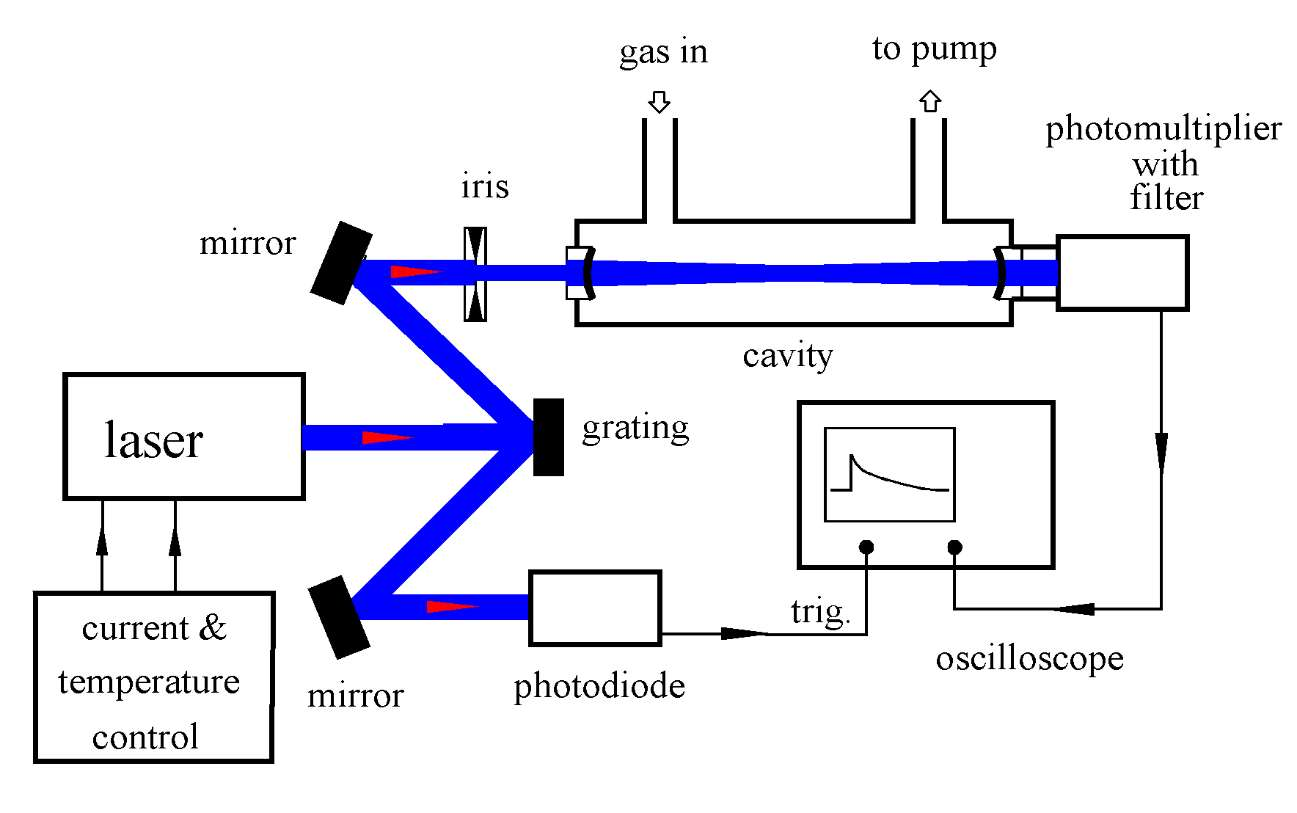
\includegraphics[width=11cm]{pictures/uklad.jpg}
    \caption{Schemat budowy układu doświadczalnego \cite{sswo}}
    \label{schem}
\end{figure}

Układ wykorzystany przy dokonywaniu pomiarów zbudowany był w oparciu o laser półprzewodnikowy. Generował on pulsy światła o długości 411 $nm$ trwające ok. 6 $ns$ z częstotliwością 10 $kHz$. Światło lasera padało na płytkę dyfrakcyjną, która pozwalała na wyeliminowanie niechcianych częstotliwości światła pochodzących z otoczenia oraz dzieliła impuls lasera na dwie części \cite{sswo}. Jedna z uzyskanych w ten sposób wiązek kierowana odpowiednio ustawionymi lustrami trafiała na fotodiodę której wyjście było podłączone do pierwszego kanału oscyloskopu. Druga z nich po przejściu przez soczewkę wpadała do rezonatora optycznego wypełnionego badaną próbką powietrza. Przy jednym z luster rezonatora znajdował się fotopowielacz mierzący natężenie światła wychodzącego przez to lustro.  Jego wyjście było podłączone do drugiego kanału oscyloskopu.

\section{Zasada działania układu badawczego} 
Uzyskane w wyniku rozszczepienia na płytce dyfrakcyjnej wiązki światła trafiały na fotodiodę i do rezonatora optycznego mniej więcej w tym samym momencie. Rezonator był skalibrowany w taki sposób, że pojawienie się w nim światła lasera powodowało wzbudzenie w nim modu drgań. Fotopowielacz przyłączony do rezonatora pozwalał na zmierzenie natężenia światła wychodzącego z rezonatora w danym momencie. Sygnał pojawiający się na kanale pierwszym oscyloskopu, czyli ten pochodzący z fotodiody, pozwalał na określenie czasu dotarcia impulsu. Sygnał z kanału drugiego oscyloskopu, czyli tego pochodzącego z fotopowielacza, pozwalał na określenie szybkości spadku natężenia światła we wnęce optycznej. Zmierzenie tej wartości pozwalało na skuteczne określenie stężenia NO2 w danej próbce w przy wykorzystaniu metody SSWO opisnanej w \ref{sswow}.

\section{Opis przeprowadzonych pomiarów}
W doświadczeniu wykorzystano próbki powietrza pobrane w laboratorium w którym przeprowadzono szereg wyładowań elektrycznych mogących wywołać zmianę stężenia $\text{NO}_{\text{2}}$ w otaczającej je atmosferze. W laboratorium pobrano próbkę powietrza z pomieszczenia przed i po przeprowadzeniu procesów, mieszaniny gazów powstałą w wyniku krótkiego i długiego wyładowania iskrowego oraz  trzech wyładowań koronowych o różnej sile. Pobrano również próbkę azotu pierwiastkowego wyparowanego z jego ciekłej fazy. 

Pomiary zaczynano od wprowadzenia badanej próbki gazu do rezonatora optycznego będącego częścią układu badawczego. Następnie włączano laser i oscyloskop po czym rozpoczynano zapis danych. Po 25 pulsach lasera przerywano działanie układu i zapisywano uzyskane wyniki. Proces przeprowadzano dla każdej badanej próbki.

\section{Format otrzymanych przeze mnie danych} 

Od prowadzącego ćwiczenia otrzymałem szereg plików o rozszerzeniu xlsx zawierających dane odczytane z oscyloskopu uzyskane dla różnych próbek jak i plik tekstowy zawierający wartości parametru sigma dla różnych częstotliwości światła dla cząsteczki $\text{NO}_{\text{2}}$. Tabela określająca który plik reprezentuje dane zebrane dla danej próbki znajdowała się w  dokumencie przekazanym przez prowadzącego ćwiczenie \cite{sswo}.

\begin{table}[h]
    \centering
    \caption{struktura otzrymanych plików}
    \label{struktura_danych}
    \resizebox{\textwidth}{!}{%
    \begin{tabular}{@{}l|l|l|l|l|l|l|@{}}
    \cmidrule(l){2-7}
     &
      Sample &
      $T$ $[s]$ &
      $ch1$ &
      $ch2$ &
      $mean$ &
      $inverted$ \\ \midrule
    \multicolumn{1}{|l|}{indeks} &
      \multicolumn{1}{c|}{\begin{tabular}[c]{@{}c@{}}numer \\ sampla\end{tabular}} &
      \multicolumn{1}{c|}{\begin{tabular}[c]{@{}c@{}}Czas w \\ sekundach\end{tabular}} &
      \multicolumn{1}{c|}{\begin{tabular}[c]{@{}c@{}}sygnał  z \\ pierwszego\\ kanału \\ oscyloskopu\end{tabular}} &
      \multicolumn{1}{c|}{\begin{tabular}[c]{@{}c@{}}sygnał z \\ drugiego\\ kanału \\ oscyloskopu\end{tabular}} &
      \multicolumn{1}{c|}{\begin{tabular}[c]{@{}c@{}}uśredniony \\ sygnał\\ z kanału\\  drugiego\end{tabular}} &
      \multicolumn{1}{c|}{\begin{tabular}[c]{@{}c@{}}sygnał \\ uśredniony \\ przemnożony \\ przez -1\end{tabular}} \\ \bottomrule
    \end{tabular}%
    }
\end{table}

\newpage

Dane w plikach xlsx były rozdzielone na sześć kolumn których opisy były nakreślone w dokumencie przekazanym przez prowadzącego ćwiczenie \cite{sswo}.

\begin{table}[h]
    \centering
    \caption{opis otrzymanych plików}
    \label{pliki}
    \resizebox{\textwidth}{!}{%
    \begin{tabular}{@{}|c|c|c|@{}}
    \toprule
    \textbf{nazwa} & \textbf{opis pochodzenia próbki}                                                                         & \textbf{nazwa pliku}   \\ \midrule
    Pure Nitrogen  & \begin{tabular}[c]{@{}c@{}}Azot cząsteczkowy\\ Odparowany z fazy ciekłej\end{tabular}                    & \textit{nitrogen.xlsx} \\ \midrule
    Air 1            & \begin{tabular}[c]{@{}c@{}}Powietrze zebrane z laboratorium \\ przed rozpoczęciem wyładowań\end{tabular} & \textit{air1.xlsx}     \\ \midrule
    Spark 1        & \begin{tabular}[c]{@{}c@{}}Mieszanina powstała w otoczeniu\\ długiego wyładowania iskrowego\end{tabular} & \textit{spark1.xlsx}   \\ \midrule
    Spark 2 & \begin{tabular}[c]{@{}c@{}}Mieszanina powstała w otoczeniu\\ krótkiego wyładowania iskrowego\end{tabular}  & \textit{spark2.xlsx} \\ \midrule
    Crone 1        & \begin{tabular}[c]{@{}c@{}}Mieszanina powstała w otoczeniu\\ słabego wyładowania koronowego\end{tabular} & \textit{crone1.xlsx}   \\ \midrule
    Crone 2 & \begin{tabular}[c]{@{}c@{}}Mieszanina powstała w otoczeniu\\ średniego wyładowania koronowego\end{tabular} & \textit{crone2.xlsx} \\ \midrule
    Crone 3        & \begin{tabular}[c]{@{}c@{}}Mieszanina powstała w otoczeniu\\ silnego wyładowania koronowego\end{tabular} & \textit{crone3.xlsx}   \\ \midrule
    Air 2          & \begin{tabular}[c]{@{}c@{}}Powietrze zebrane z laboratorium \\ po przeprowadzeniu wyładowań\end{tabular} & \textit{air2.xlsx}     \\ \bottomrule
    \end{tabular}%
    }
\end{table}

\section{Charakterystyka uzyskanych sygnałów}
\begin{wrapfigure}{r}{4cm}
    \centering
    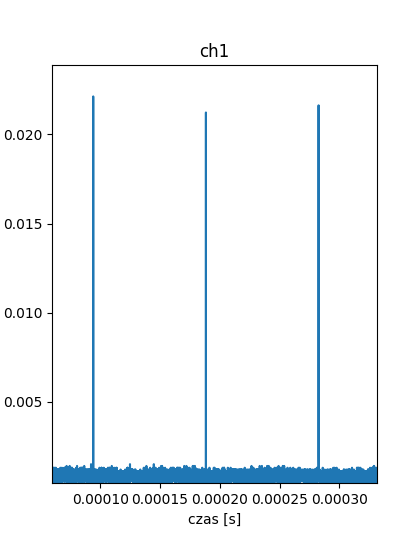
\includegraphics[width=4cm]{pictures/ch1_1.png}
    \caption{sygnał ch1 z pliku  \textit{air1.xlsx}}
    \label{ch1_1}
\end{wrapfigure}

Zachowanie sygnałów zebranych z pierwszego kanału oscyloskopu było różne dla różnych plików. Dla plików \textit{nitrogen.xlsx}, \textit{spark1.xlsx}, \textit{crone1.xlsx} i \textit{air1.xlsx} w danych zapisanych z pierwszego kanału oscyloskopu dało się zaobserwować bardzo wyraźne i wąskie skoki napięcia. Skoki te występowały w równych odstępach od siebie, i w każdej serii pomiarowej było ich 25. Korespondowały one z wykryciem przez fotodiodę impulsu wygenerowanego przez laser.
W danych z kanału pierwszego w plikach \textit{spark2.xlsx} \textit{spark3.xlsx}, \textit{crone2.xlsx} oraz \textit{air2.xlsx} dało się zaobserwować dwa napięcia pomiędzy którymi sygnał gwałtownie przeskakiwał. Przeskoki napięcia występowały w równych odstępach, a czas przez jaki sygnał pozostawał na danym napięciu nie zmieniała się pomiędzy kolejnymi zmianami. W obydwu
\newpage 
\begin{wrapfigure}{l}{4cm}
    \centering
    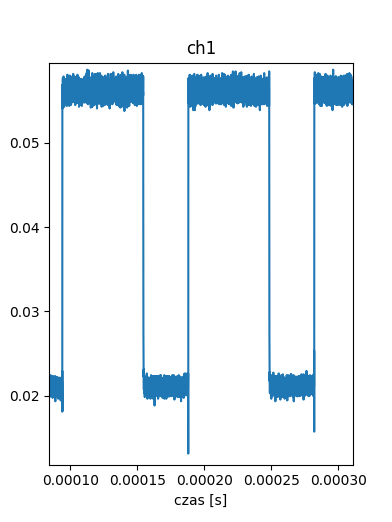
\includegraphics[width=4cm]{pictures/ch1_2.png}
    \caption{sygnał ch1 z pliku  \textit{air2.xlsx}}
    \label{ch1_2}
\end{wrapfigure}
przypadkach dane zebrane z pierwszego kanału oscyloskopu charakteryzował bardzo niski poziom szumu. 
W celu uzyskania reprezentacji natężenia światła padającego na będący częścią układu badawczego fotopowielacz sygnał z drugiego kanału oscyloskopu odpowiednio uśredniono i pomnożono przez -1 \cite{strona}. Dalej tak spreparowany sygnał będę określał sygnałem przetworzonym. Uzyskane w ten sposób dane charakteryzował znacząco wyższy poziom szumu od tego występującego w sygnale pobranym z kanału pierwszego. Pozostawały one spójne pomiędzy seriami i dało się w nich zaobserwować gwałtowne skoki w natężeniu, po których sygnał eksponencjalnie spadał do wartości sprzed skoku. W  każdej analizowanej serii danych występowało 25 takich pików. W przypadku danych z plików \textit{nitrogen.xlsx}, \textit{spark1.xlsx}, \textit{crone1.xlsx} i \textit{air1.xlsx} pokrywały się one w czasie z pikami obserwowanymi na kanale pierwszym. W przypadku plików \textit{spark2.xlsx} \textit{spark3.xlsx}, \textit{crone2.xlsx} otrzymane piki te pokrywały się z przeskokiem napięcia kanale pierwszym z niskiego na wysokie. Na podstawie tej zgodności można stwierdzić że wzrost napięcia na kanale pierwszym wiązał się z wykryciem przez podłączoną do niego fotodiodę impulsu lasera. Jest to zachowanie zgodne z przewidywaniami teoretycznymi. W obu przypadkach uzyskane dane wyglądały na prawidłowe, jednak wartość wyjściowa (występujące na kanale zaraz przed pojawieniem się skoku) było nieznacznie mniejsze od 0. Po przesunięciu danych w taki sposób, by wartość wyjściowa wynosiła  0 dane stawały się zgodne z przewidywaniami teoretycznymi.

\begin{figure}[h]
    \centering
    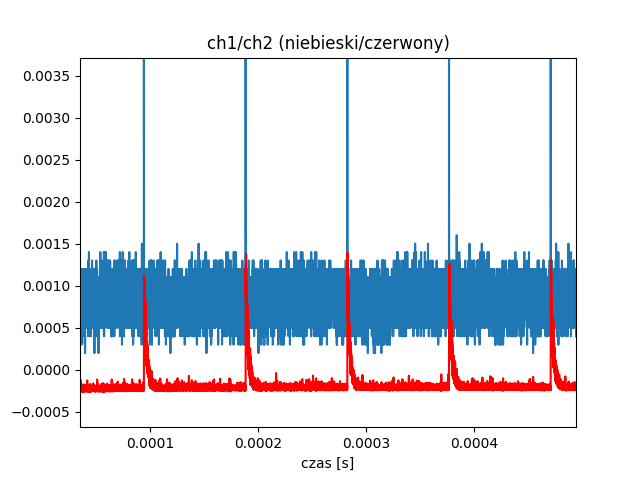
\includegraphics[width=6cm]{pictures/ch2_1.png}
    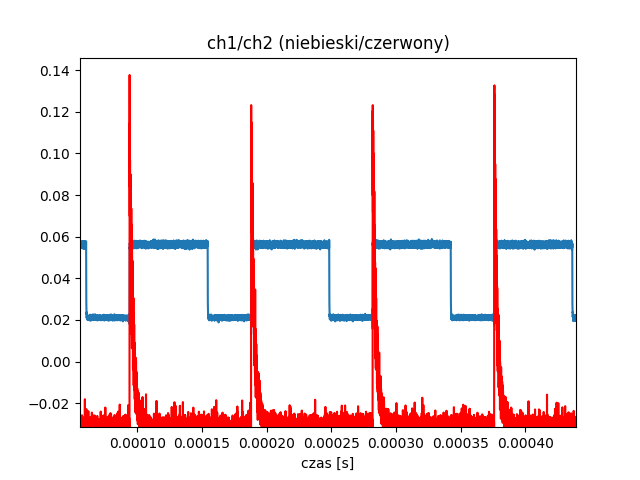
\includegraphics[width=6cm]{pictures/ch2_2.png}
    \caption{sygnały ch2 i ch1 z plików \textit{air2.xlsx}  i \textit{air1.xlsx}}
    \label{ch2_1}
\end{figure}

\section{Metoda analizy danych}
\label{method}
Analizę danych rozpocząłem od  wprowadzenia danych do napisanego przez mnie programu w pythonie. 
Wyznaczanie stężenie $\text{NO}_{\text{2}}$ dla danej próbki rozpoczynałem od przeanalizowania sygnału z kanału pierwszego.  W celu ujednolicenia charakterystyki danych na podstawie tych sygnałów tworzyłem nową serię o takiej samej ilości rekordów. Każdy z nich zawierał różnicę wartości pomiędzy wartością napięcia na kanale pierwszym dla indeksu odpowiadającemu indeksowi nowego rekordu a wartością go poprzedzającą. W uzyskanej w ten sposób serii danych dla każdego pliku występowały wyraźne i wąskie piki pojawiające się dla indeksów dla których w danych zebranych z kanału pierwszego pojawiał się gwałtowny skok napięcia.
Wyznaczenia lokalizacji tych pików dokonywałem poprzez znalezienie punktów dla których wartości nowo uzyskanej serii danych przekraczały pewną wartość graniczną $V_{gran}$. Wartość tą wyznaczyłem ze wzoru:
\begin{equation}
    \label{tresh}
    V_{gran} = \frac{maksymalna\; wartosc\; danych - srednia\; wartosc\; danych}{3.5}
\end{equation}
Taką metodę wyznaczania wartości granicznej dobrałem arbitralnie, ale zweryfikowałem jej skuteczność poprzez wizualną weryfikację jej rezultatów dla każdej badanej serii danych.
\begin{figure}[h]
    \centering
    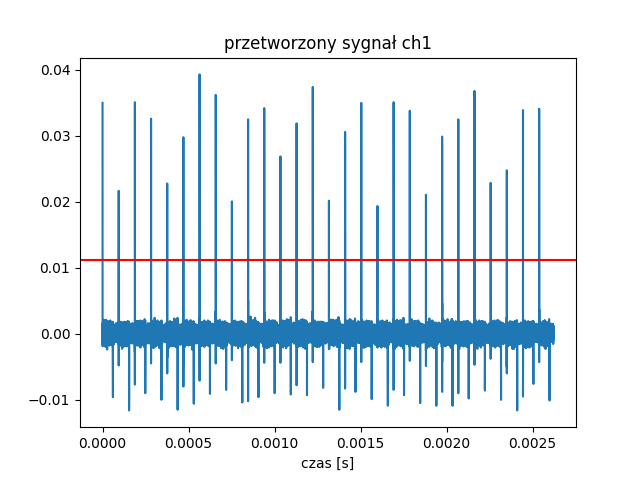
\includegraphics[width=11cm]{pictures/thresh.png}
    \caption{przykładowy przetworzony sygnał ch1 z zaznaczoną wartością graniczną}
    \label{tresh}
\end{figure}
Jeśli powyżej wartości granicznej zawierało się kilka następujących po sobie punktów wybierałem ten o najwyższej wartości, a pozostałe odrzucałem. Do uzyskanych w ten sposób indeksów dopisywałem ostatni index serii po czym zapisywałem rezultaty. 
Na podstawie uzyskanych wcześniej punktów dzieliłem przetworzony sygnał z kanału drugiego na przedziały. Następnie ażdy z nich transformowałem w taki sposób by czas odpowiadający pierwszemu pomiarowi wynosił 0. Wartości sygnału dla każdego występującego czasu pomiaru uśredniałem. Następnie znajdowałem najwyższą wartość z pośród uzyskanych w ten sposób danych i odrzucałem wartości występujące przed nią.  W ten sposób uzyskiwałem uśrednioną  reprezentacje przetworzonego sygnał z kanału 2 zawierającą tylko eksponencjalny spadek wartości do wartości wyjściowej. Do tak spreparowanych danych dopasowywałem funkcje zależą od parametrów $a$ i $b$: 
\begin{equation}
    \label{exp}
    f(t) = a e^{\frac{-t}{b}} + c
\end{equation}
Jako początkową wartość $a$ przyjmowałem maksymalną wartość uzyskaną w przedziale, a początkową wartość parametru b wyliczałem ze wzoru:

\begin{equation}
    \label{binit}
    b_{init} = \frac{-t[80]}{\ln{\frac{V[80]}{a}}}
\end{equation}

Gdzie $t[80]$ i $V[80]$ odpowiadają kolejno 80 pomiarowi czasu i 80 pomiarowi przetworzonego sygnału na kanale drugim w badanym przedziale.  Wzór ten został przeze mnie wybrany arbitralnie, ale małe odchylenia parametrów dopasowanych przy jego pomocy świadczył że wyznaczał on odpowiednią wartość początkową parametru $b$. Uzyskane w ten sposób parametry początkowe gwarantowały, że funkcja od której rozpoczynałem dopasowanie w przynajmniej dwóch punktach zgadzała się z zadanymi wartościami.
Wartości $b$ oraz związane z nimi oniepewności zapisywałem. Proces powtórzyłem dla wszystkich dostarczonych plików.
Wykorzystany przez mnie program dołączyłem jako załącznik do raportu

\section{Interpretacja dopasowanych parametrów oraz dalsza analiza danych}

Po uzyskaniu wyników działania programu uzyskane rezultaty przepisywałem do arkusza kalkulacyjnego. Uzyskane w wyniku dopasowania wartości $b$ odpowiadają parametrom $\tau$ zdefiniowanych w paragrafie \ref{sswow}. Azot cząsteczkowy wyparowany z ciekłej fazy nie powinien zawierać $\text{NO}_{\text{2}}$, w takim razie $b$ uzyskaną dla tej próbki możemy traktować jako wartość $\tau_0$. Wartość sigma dla światła częstotliwości  światła generowanej przez laser jesteśmy w stanie określić stężenie $\text{NO}_{\text{2}}$ w badanych próbkach możemy wyznaczyć ze wzoru \ref{stęż}.  Uzyskanie stężenie określa ilość cząsteczek substancji w centymetrze sześciennym powietrza.  
Stężenie wyrażone w gramach na centymetr sześcienny $d$ jesteśmy w stanie określić na podstawie wzoru
\begin{equation}
    \label{dens}
    d = \frac{N m_a}{M_u}
\end{equation}
Gdzie:
\begin{itemize}
    \item $m_a$ - masa atomowa
    \item $N$ - wyliczone wcześniej stężenie
    \item $M_u$ - stała masy molowej
\end{itemize}
 Znając wartość $d$ jesteśmy w stanie określić stężęnei $\text{NO}_{\text{2}}$ wyrażone w ppb $C$ wykorzystując wzór
\begin{equation}
    \label{ce}
    C=\frac{d}{d_a} 10^9
\end{equation}
gdzie $d_a$ jest gęstością powietrza w laboratorium
Podstawiając wzór \ref{ce} do \ref{dens} otrzymamy wyrażenie pozwalający określić stężenie wyrażone w ppb na podstawie stężenia wyrażonego w cząsteczkach na centymetr sześcienny
\begin{equation}
    \label{cer}
    C = N \frac{m_a}{d_a M_u}10^9
\end{equation}

Wykorzystany przez mnie arkusz kalkulacyjny dołączyłem do raportu jako złącznik


\section{Obliczanie niepewności pomiarowych}

Jako niepewność pomiaru $\tau$ przyjąłem niepewności uzyskane przy dowpasowywaniu parametru $b$ dla danej próbki. Niepewność stężenia NO2 w próbce wyliczyłem wykorzystując metodę różniczki zupełnej
\begin{equation}
    \label{niept}
    \Delta N = \frac{1}{c \sigma} \left(\frac{\Delta \tau}{\tau^2} - \frac{\Delta \tau_0}{\tau_0^2} \right)
\end{equation}
Tą samą metodę wykorzystałem do wyznaczenia niepewności stężenie wyrażanego w ppb:
\begin{equation}
    \label{niepn}
    \Delta C = \Delta N \frac{m_a}{d_a M_u}10^9
\end{equation}


\section{Uzyskane wyniki}
Wartości $\tau$ wraz z związanymi z nimi odchyleniami standardowymi przepisałem do arkusza kalkulacyjnego, po czym przy jego pomocy obliczyłem szukane stężenia. Przy wykonywaniu obliczeń za prędkość światła przyjąłem $29979245800$ $[cm/s]$ \cite{c}  a za stałą Masy molowej $6.02214076 10^{23}$ $[g/mol]$ \cite{c}  . Masę atomową cząsteczki $\text{NO}_{\text{2}}$ przyjąłem $46u$. Wartości $\sigma$ odczytałem z pliku \textit{NO2.txt} uzyskująć $6.362 10^{19}$ $[cm^2]$ a za gęstość powietrza $0.001225$ $[g/cm^3]$ \cite{air}. Uzyskane przeze mnie przedstawiłem w tabeli.


\begin{table}[h]
    \caption{uzyskane wyniki}
    \label{tab:my-table}
    \resizebox{\textwidth}{!}{%
    \begin{tabular}{|l|l|l|l|l|l|l|l|l|l|l|}
    \hline
    próbka &
      $\tau$ $[s]$ &
      $\Delta \tau$ $[s]$ &
      $\alpha$ $\left[\frac{1}{cm}\right]$ &
      $\Delta \alpha$ $\left[\frac{1}{cm}\right]$ &
      $\frac{N}{cm^3}$   $\left[\frac{1}{cm^3}\right]$ &
      $\frac{\Delta N}{cm^3}$   $\left[\frac{1}{cm^3}\right]$ &
      \textbf{$\frac{g}{cm^3}$} &
      \textbf{$\Delta \frac{g}{m^3}$} &
      \textbf{$ppb$} &
      \textbf{$\Delta ppb$} \\ \hline
    nitrogen & 2.40E-06 & 3.32E-09 &          &          &          &          &          &          &       &     \\ \hline
    air1     & 2.34E-06 & 3.05E-09 & 3.09E-07 & 3.78E-08 & 4.86E+11 & 5.95E+10 & 3.71E-11 & 4.54E-12 & 30    & 4   \\ \hline
    air2     & 2.35E-06 & 2.94E-09 & 3.05E-07 & 3.71E-08 & 4.80E+11 & 5.83E+10 & 3.66E-11 & 4.46E-12 & 30    & 4   \\ \hline
    crone1   & 1.46E-06 & 4.09E-09 & 8.90E-06 & 8.31E-08 & 1.40E+13 & 1.31E+11 & 1.07E-09 & 9.98E-12 & 873   & 8   \\ \hline
    crone2   & 5.28E-07 & 1.58E-09 & 4.93E-05 & 2.09E-07 & 7.74E+13 & 3.28E+11 & 5.91E-09 & 2.51E-11 & 4828  & 20  \\ \hline
    crone3   & 2.01E-06 & 2.63E-09 & 2.67E-06 & 4.10E-08 & 4.20E+12 & 6.44E+10 & 3.21E-10 & 4.92E-12 & 262   & 4   \\ \hline
    spark1   & 4.58E-07 & 3.10E-09 & 5.90E-05 & 5.14E-07 & 9.27E+13 & 8.07E+11 & 7.08E-09 & 6.17E-11 & 5782  & 50  \\ \hline
    spark2   & 2.01E-07 & 2.68E-09 & 1.52E-04 & 2.23E-06 & 2.39E+14 & 3.51E+12 & 1.82E-08 & 2.68E-10 & 14890 & 219 \\ \hline
    \end{tabular}%
    }
\end{table}

\newpage

\begin{figure}[h]
    \centering
    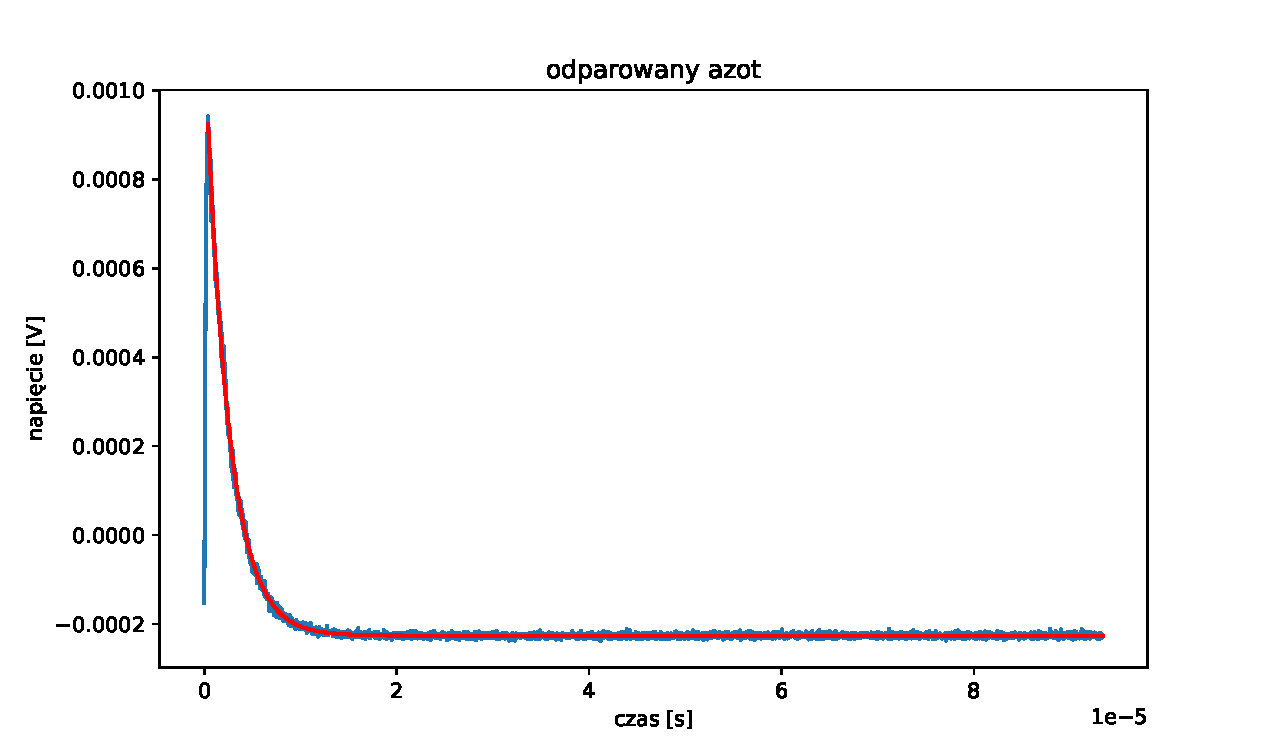
\includegraphics[width=6cm]{nitrogen.pdf}
    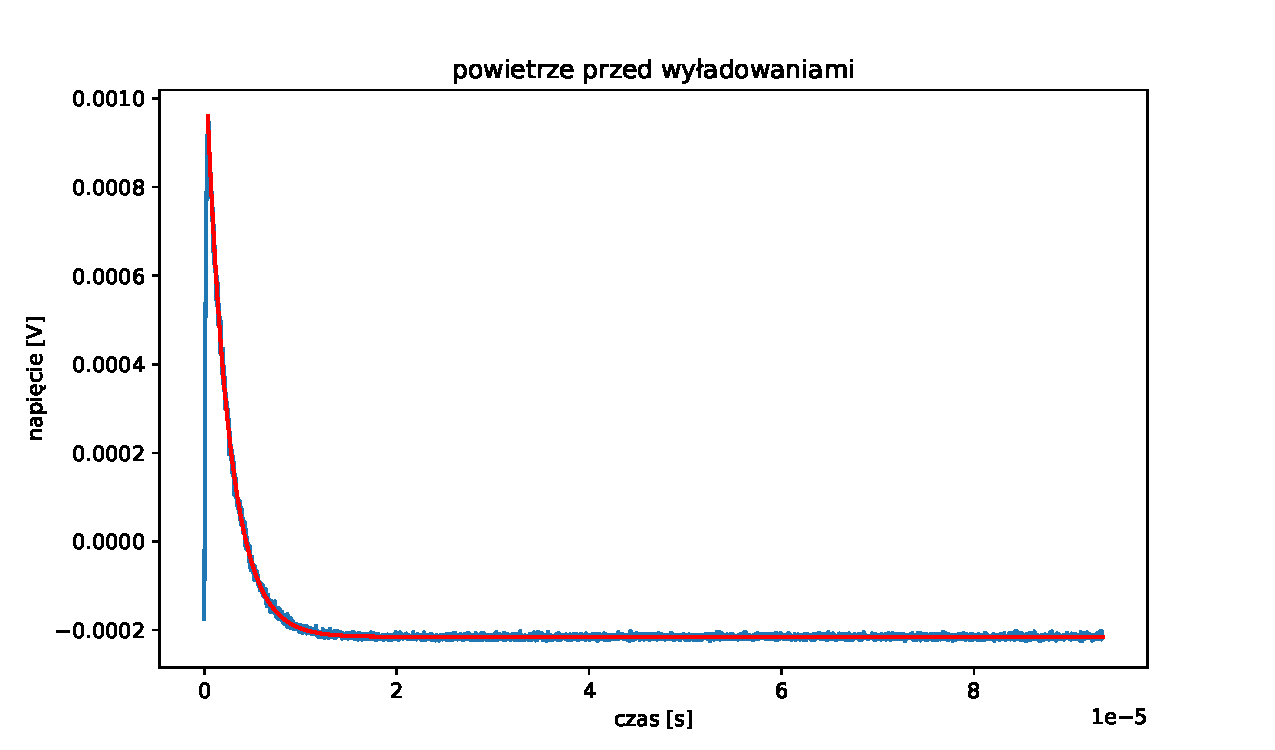
\includegraphics[width=6cm]{air1.pdf}
    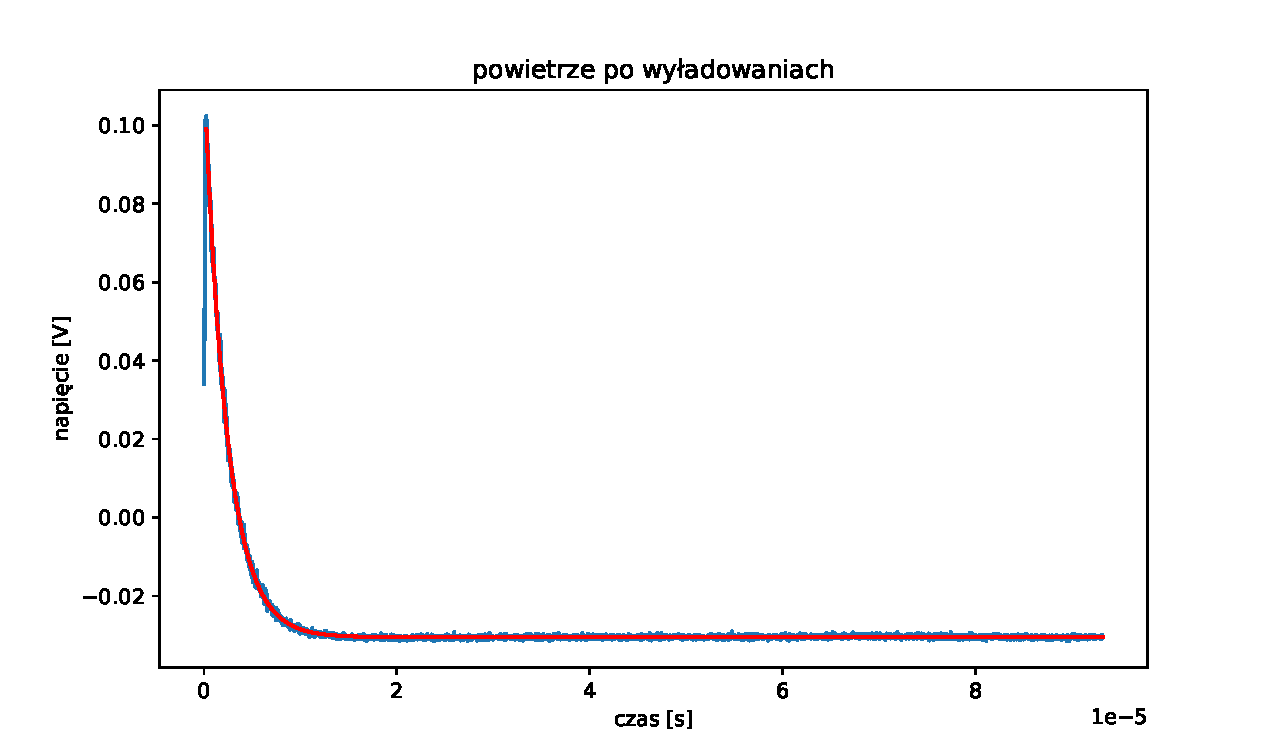
\includegraphics[width=6cm]{air2.pdf}
    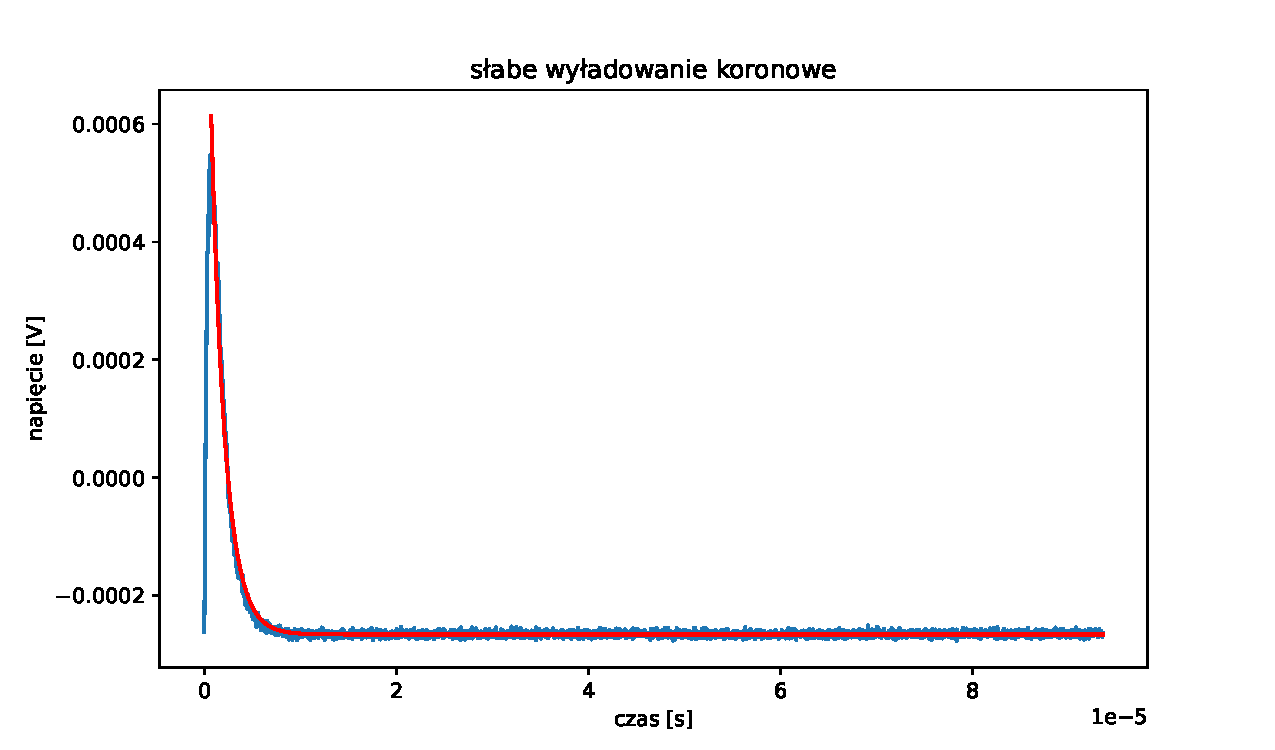
\includegraphics[width=6cm]{crone1.pdf}
    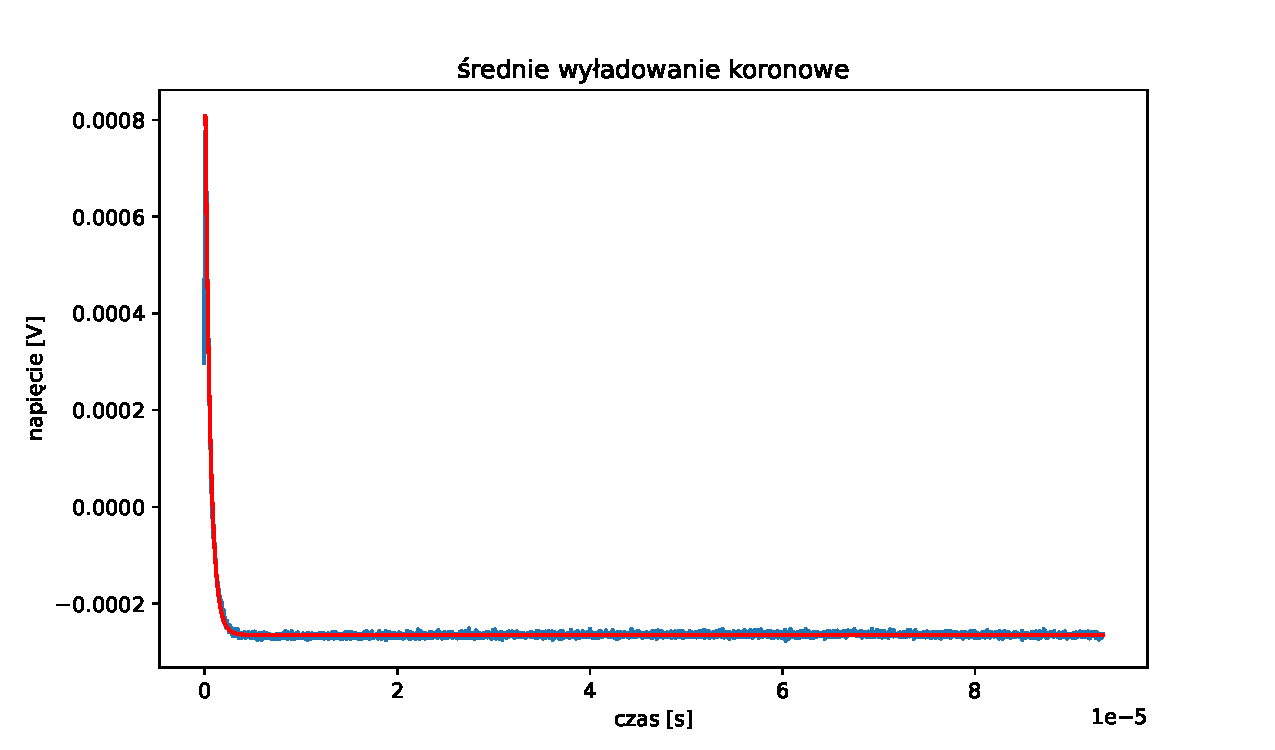
\includegraphics[width=6cm]{crone2.pdf}
    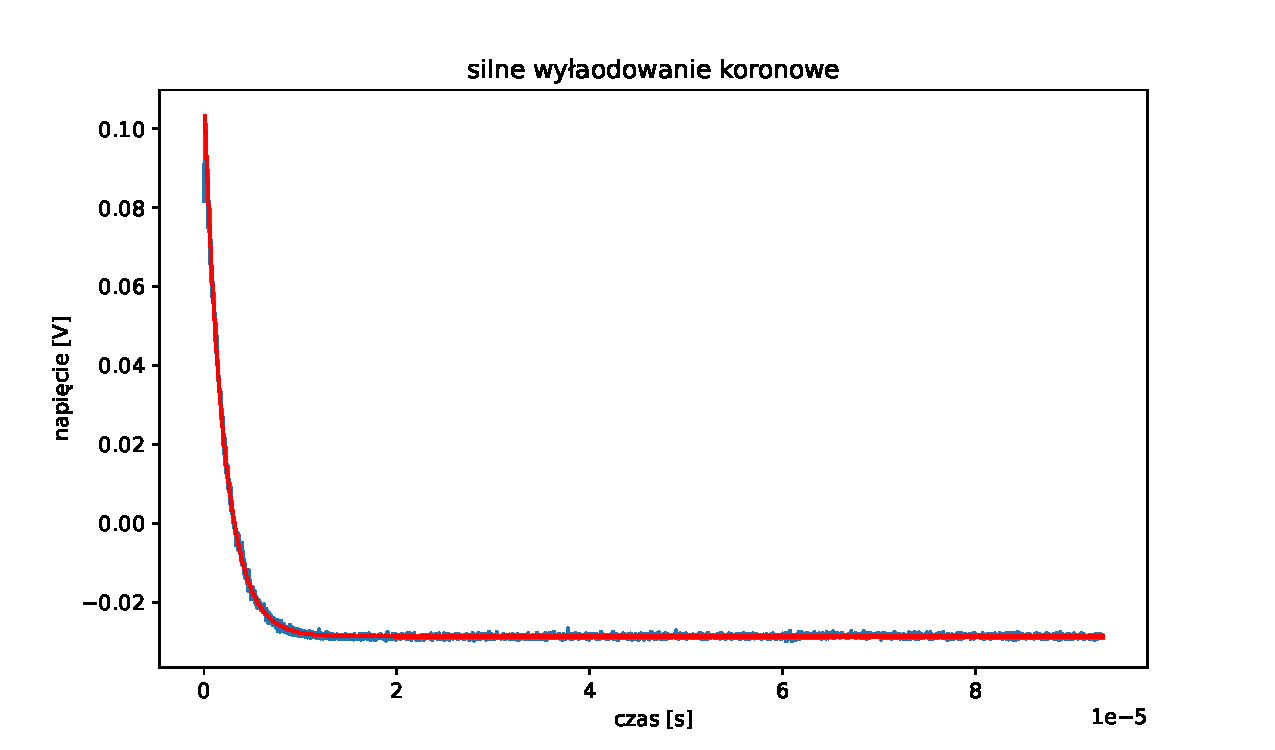
\includegraphics[width=6cm]{crone3.pdf}
    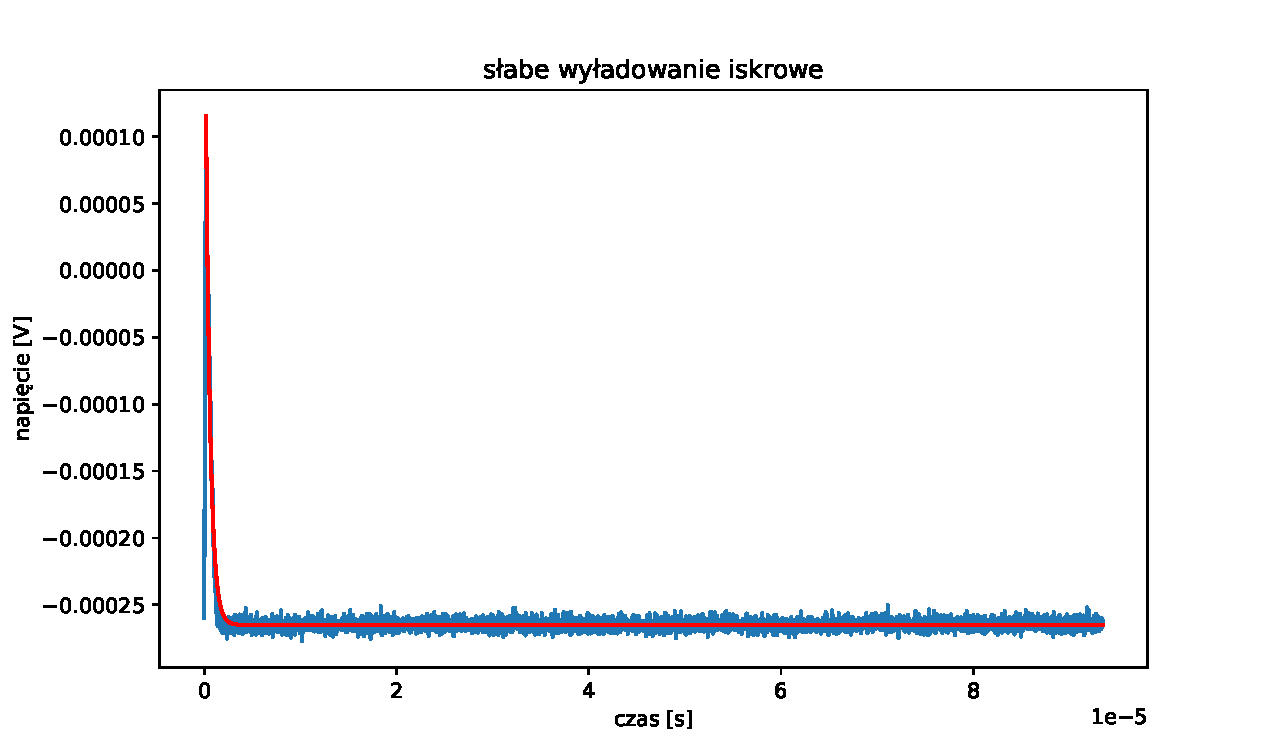
\includegraphics[width=6cm]{spark1.pdf}
    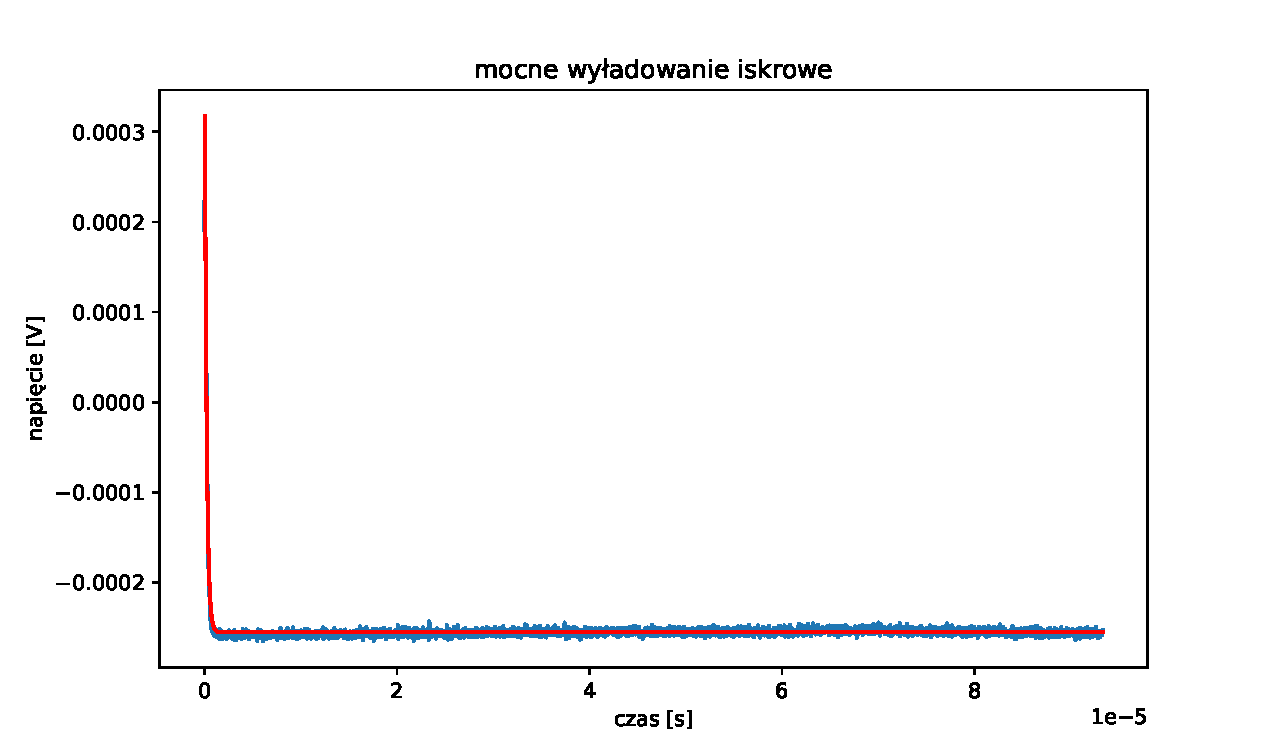
\includegraphics[width=6cm]{spark2.pdf}
    \caption{Uzyskane uśrednione sygnały wraz z dopasowanymi krzywymi}
    \label{ch2_1}
\end{figure}

\newpage

\section{Dyskusja uzyskanych wyników}
Zarówno otrzymane wartości $\tau$ jak i wyliczone na ich podstawie stężenie w większości przypadków okazały się być zgodne z przewidywaniami teoretycznymi. W powietrzu laboratorium stężenie dwutlenku azotu wynosiło kilkadziesiąt ppb. W badanych mieszaninach gazów powstałych w wyładowaniach stężenie to wynosiło kilka lub kilkanaście tysięcy ppb.  Wartość $\tau_0$ wyliczona z danych uzyskanych dla próbki odparowanego azotu okazała się być najwyższa. Jest to zachowanie zgodne z przewidywaniami, ponieważ próbka ta powinna nie zawierać w sobie cząsteczek $\text{NO}_{\text{2}}$. W próbkach powietrza pobranego z laboratorium przed i po rozpoczęciu pomiarów stężenie $\text{NO}_{\text{2}}$ było takie samo . Badane stężenie okazało się być znacząco wyższe w próbkach pobranych z otoczenia procesów przeprowadzonych w laboratorium. Są to rezultaty zgodne z przewidywaniami. Wspomniane procesy powodują powstanie $\text{NO}_{\text{2}}$ w powietrzu, jednak powstałego w ten sposób gazu jest zbyt mało by znacząco zwiększyć jego stężenie w atmosferze je otaczającej.

Zgodne z przewidywaniami okazała się również zależność stężenia $\text{NO}_{\text{2}}$ od natężenia wyładowania iskrowego z którego otoczenia ją pobrano. Wraz ze wzrostem energii wyładowania należało się spodziewać wzrostu stężenia dwutlenku azotu w wytworzonej przez nie mieszaninie gazów. W konsekwencji w próbce powietrza pobranego z otoczenia krótkiego wyładowania iskrowego stężenie $\text{NO}_{\text{2}}$ było niższe od tego w próbce pobranej z otoczenia długiego wyładowania iskrowego.

Niezgodną z przewidywaniami okazała się być zależność stężenia $\text{NO}_{\text{2}}$ w próbce od natężenia wyładowania koronowego. Stężenie dwutlenku azotu okazało się być najniższe dla najsilniejszego wyładowania, a najwyższe dla wyładowania o średniej sile.

\section{Dyskusja błędów pomiarowych oraz niezgodności z przewidywaniami}
Dla każdej z badanych próbek wyznaczone przez mnie niepewności wartości $\tau$ były dwa lub trzy rzędy wielkości mniejsze od otrzymanej wartości parametru. Świadczy to dużej dokładności przeprowadzonych pomiarów oraz o dobrej skuteczności dopasowania. Uzyskane przez mnie wartości $\tau$ wraz ze związanymi z nimi niepewnościami można traktować jako miarodajne. We wszystkich przypadkach okazały się one wystarczające by na ich podstawie skutecznie określić stężenie $\text{NO}_{\text{2}}$ w odpowiadającej im próbce. Potencjalny negatywny wpływ na wartości niepewności parametrów pochodzący od stosunkowo dużego szumu występującego w sygnale zebranym z drugiego kanału oscyloskopu został skutecznie wykluczony poprzez uśrednienie danych z wyznaczonych przedziałów.
Niepewności obydwu wyliczonych stężeń dla próbek w których dopasowanie wartości $\tau$ były zbliżone do $\tau_0$ stanowiły większy ułamek związanej z nimi wartości niż dla pozostałych próbek. Uzyskane przez mnie niepewności związane z pomiarem $\tau$ okazały się być jednak na tyle małe że możliwe było miarodajne wyznaczenie ich stężenia $\text{NO}_{\text{2}}$.  Zwiększony stosunek wartosci niepewności do wyniku wynikał z zachowania wzoru \ref{niept}  dla bliskich sobie wartości $\tau$ i $\tau_0$.  Jako że wartość  i niepewność stężenia dwutlenku azotu wyrażona w ppb zależy liniowo od kolejno wartości i niepewności  stężenia wyrażonego cząstkach na $cm^3$ analogiczny problem dotyczył stężenia wyrażonego w ppb.
Dla pozostałych próbek niepewności stężeń były dwa lub trzy rzędy wielkości mniejsze od ich wartości. Dla tych próbek uzyskane stężenia również można uznać za miarodajne
Uzyskane przeze mnie stężenia dla próbek pobranych z otoczeń wyładowań koronowych okazały się być niezgodne z przewidywaniami teoretycznymi. W ich przypadku stężenie dwutlenku azotu w próbce pobranej z otoczenia procesu powinno wzrastać wraz ze wzrostem intensywności procesu. W próbkach pobranych z otoczeń wyładowań koronowych najniższe stężenie $\text{NO}_{\text{2}}$ uzyskałem dla próbki z otoczenia najsilniejszego wyładowania. Niezgodność ta mogła być spowodowana błędem przy dopasowywaniu krzywych do otrzymanych danych, jednak niskie odchylenia standardowe dopasowani sugerują że były one przeprowadzone poprawnie. Zaistniałe odstępstwo mogło być również spowodowane wykorzystaniem przez mnie błędnej metody wyliczania stężenia $\text{NO}_{\text{2}}$ lub złym oznaczeniem plików przez osobę zbierającą wyniki. 


\addcontentsline{toc}{section}{Podsumowanie}
\section*{Podsumowanie}
Wyliczone przez mnie stężenia dwutlenku azotu w badanych próbkach powietrza okazały się być częściowo zgodne z przewidywaniami teoretycznymi. Otrzymane przez mnie uśrednione wartości parametrów $\tau$ uzyskane w wyniku dopasowani krzywych charakteryzowały niskie niepewności pomiarowe. Wyliczone na ich podstawie stężenia $\text{NO}_{\text{2}}$ wyrażone w cząstkach na $cm^3$ i w ppb miały odpowiednie rzędy wielkości. Wyliczone przeze mnie niepewności pomiarowe okazały się być na tyle małe, że korelujące z nimi dane uznałem za miarodajne. Dla próbek o małej zawartości $\text{NO}_{\text{2}}$ stosunek niepewności do związanej z nią wartości okazał się być wyższy od tego uzyskanego dla pozostałych próbek. Nie ma to jednak wpływu na użyteczność rezultatów. W uzyskanych przez mnie wynikach da się zaobserwować korelację pomiędzy stężeniem $\text{NO}_{\text{2}}$ w próbce a natężeniem wyładowania iskrowego z którego otoczenia była ona pobrana. Takiej relacji nie da się jednak zaobserwować w wynikach uzyskanych dla próbek z otoczeń wyłaodwań koronowych. Jest to zachowanie niezgodne z przewidywaniami teoretycznymi. Jednak nawet w obliczu zaobserwowanych niezgodności metoda SSWO okazała się być bardzo skuteczna w dokładnym wykrywaniu stężeń nawet śladowych ilości konkretnych cząsteczek w ośrodkach

\newpage
\bibliographystyle{unsrt}
\bibliography{References}


\end{document}


